%
% This is a borrowed LaTeX template file for lecture notes for CS267,
% Applications of Parallel Computing, UC Berkeley EECS Department.
% Now being used for Carnegie Mellon University's 10-725/36-725 
% Convex Optimization course taught by Ryan Tibshirani.  When
% preparing LaTeX notes for this class, please use this template. 
%
% To familiarize yourself with this template, the body contains
% some examples of its use.  Look them over.  Then you can
% run LaTeX on this file.  After you have LaTeXed this file then
% you can look over the result either by printing it out with
% dvips or using xdvi. "pdflatex template.tex" should also work.
%

\documentclass[twoside]{article}
\setlength{\oddsidemargin}{0.25 in}
\setlength{\evensidemargin}{-0.25 in}
\setlength{\topmargin}{-0.6 in}
\setlength{\textwidth}{6.5 in}
\setlength{\textheight}{8.5 in}
\setlength{\headsep}{0.75 in}
\setlength{\parindent}{0 in}
\setlength{\parskip}{0.1 in}

%
% ADD PACKAGES here:
%
\usepackage{bm}
\usepackage{amsmath,amsfonts,graphicx}

%
% The following commands set up the lecnum (lecture number)
% counter and make various numbering schemes work relative
% to the lecture number.
%
\newcounter{lecnum}
\renewcommand{\thepage}{\thelecnum-\arabic{page}}
\renewcommand{\thesection}{\thelecnum.\arabic{section}}
\renewcommand{\theequation}{\thelecnum.\arabic{equation}}
\renewcommand{\thefigure}{\thelecnum.\arabic{figure}}
\renewcommand{\thetable}{\thelecnum.\arabic{table}}

%
% The following macro is used to generate the header.
%
\newcommand{\lecture}[4]{
   \pagestyle{myheadings}
   \thispagestyle{plain}
   \newpage
   \setcounter{lecnum}{#1}
   \setcounter{page}{1}
   \noindent
   \begin{center}
   \framebox{
      \vbox{\vspace{2mm}
    \hbox to 6.28in { {\bf MATH 680: Computation Intensive Statistics \hfill Winter 2018} }
       \vspace{4mm}
       \hbox to 6.28in { {\Large \hfill Lecture #1: #2  \hfill} }
       \vspace{2mm}
       \hbox to 6.28in { {\it Lecturer: #3 \hfill Scribes: #4} }
      \vspace{2mm}}
   }
   \end{center}
   \markboth{Lecture #1: #2}{Lecture #1: #2}

   {\bf Note}: {\it LaTeX template courtesy of UC Berkeley EECS dept.}

   {\bf Disclaimer}: {\it These notes have not been subjected to the
   usual scrutiny reserved for formal publications. They may be
   distributed outside this class only with the permission of the
   Instructor.} \vspace*{4mm}
}
%
% Convention for citations is authors' initials followed by the year.
% For example, to cite a paper by Leighton and Maggs you would type
% \cite{LM89}, and to cite a paper by Strassen you would type \cite{S69}.
% (To avoid bibliography problems, for now we redefine the \cite command.)
% Also commands that create a suitable format for the reference list.
\renewcommand{\cite}[1]{[#1]}
\def\beginrefs{\begin{list}%
        {[\arabic{equation}]}{\usecounter{equation}
         \setlength{\leftmargin}{2.0truecm}\setlength{\labelsep}{0.4truecm}%
         \setlength{\labelwidth}{1.6truecm}}}
\def\endrefs{\end{list}}
\def\bibentry#1{\item[\hbox{[#1]}]}

%Use this command for a figure; it puts a figure in wherever you want it.
%usage: \fig{NUMBER}{SPACE-IN-INCHES}{CAPTION}
\newcommand{\fig}[3]{
			\vspace{#2}
			\begin{center}
			Figure \thelecnum.#1:~#3
			\end{center}
	}
% Use these for theorems, lemmas, proofs, etc.
\newtheorem{theorem}{Theorem}[lecnum]
\newtheorem{lemma}[theorem]{Lemma}
\newtheorem{proposition}[theorem]{Proposition}
\newtheorem{claim}[theorem]{Claim}
\newtheorem{corollary}[theorem]{Corollary}
\newtheorem{definition}[theorem]{Definition}
\newenvironment{proof}{{\bf Proof:}}{\hfill\rule{2mm}{2mm}}

% **** IF YOU WANT TO DEFINE ADDITIONAL MACROS FOR YOURSELF, PUT THEM HERE:

\newcommand\E{\mathbb{E}}
\newcommand\R{\mathbb{R}}

\begin{document}
%FILL IN THE RIGHT INFO.
%\lecture{**LECTURE-NUMBER**}{**DATE**}{**LECTURER**}{**SCRIBE**}
\lecture{19}{March 21}{Lecturer: Yi Yang}{Zafarali Ahmed, Ismaila Diedhiou Balde, David Fleischer}
%\footnotetext{These notes are partially based on those of Nigel Mansell.}

% **** YOUR NOTES GO HERE:

% Some general latex examples and examples making use of the
% macros follow.  
%**** IN GENERAL, BE BRIEF. LONG SCRIBE NOTES, NO MATTER HOW WELL WRITTEN,
%**** ARE NEVER READ BY ANYBODY.

\section{Lasso}


\subsection{Two Source of Inspiration for the Lasso}

\begin{enumerate}
	\item Non-negative Garrote~\cite{B95}: The non-negative Garrote is defined by a multiple-step process. First, solve the ordinary least-squares regression problem
	\begin{equation*}
		\widehat\beta^\text{ols} = \underset{\beta \in \R^p}{\text{arg min~}} \| {\bf y} - {\bf X}\beta \|^2_2,
	\end{equation*}
	
	for $\widehat\beta^\text{ols} = \left(\widehat\beta^\text{ols}_1, ..., \widehat\beta^\text{ols}_p \right)^T$. Next, use the OLS estimate to define the (non-negative Garrote) constrained minimization problem (with respect to $c_j$)
	\begin{equation*}
		\text{Minimize} \quad \| {\bf y} - \sum^p_{j = 1}  {\bf X}_j \widehat\beta^\text{ols}_j c_j \|^2_2 \quad \text{subject to}
	\end{equation*}	
	\begin{equation*}
		\sum^p_{j = 1} c_j \leq B \quad \text{and} \quad c_j \geq 0~\forall\,j.
	\end{equation*}	
	
	where $B \in \R^+$ is a tuning parameter similar to $\lambda$ in the unconstrained Lasso problem, or $t$ in the constrained Lasso problem. Then, the non-negative Garrote solution is defined by scaling the OLS solution by the solutions $\widehat c_j$ to the above minimization problem. In particular,
	\begin{equation*}
		\widehat\beta^\text{garrote}_j = \widehat c_j \widehat \beta^\text{ols}_j.
	\end{equation*}
	
	\item Wavelet shrinkage~\cite{DJ95}: Set $y_i = \mu_i + \epsilon_i$, for $\epsilon_i \sim \mathcal N(0, 1)$, $i = 1, ..., n$. Then, define the estimate $\widehat\mu_i$ of $\mu_i$ as the solution to the unconstrained minimization problem
	\begin{equation*}
		\widehat\mu_i = \underset{\mu}{\text{arg min~}} \left\{ \frac{1}{2} \left(y_i - \mu\right)^2 + \sqrt{2\log n} |\mu| \right\}
	\end{equation*}
\end{enumerate}

\subsubsection{Non-Negative Garrote (Breiman, 1995, Technometrics)}

``Much work and research have gone into subset selection regression, but the basic method remains flawed by its relative lack of accuracy and instability. Subset regression either zeros a coefficient, it is not in the selected subsets, or inflates it. Ridge regression gains its accuracy by selective shrinking.''

``Methods that select subsets, are stable, and shrink are needed.''

The garrote eliminates some variables, shrinks others, and is relatively stable (compared with the subset selection algorithm). 

The non-negative garrote depends on both the sign and the magnitude of the OLS estimates. OLS estimates may behave poorly in some settings, such as overfit or highly correlated covariates. The non-negative garrote may suffer as a result.

Tibshirani proposed the LASSO with the goal to avoid the explicit use of the OLS estimates, as used in the non-negative garrote algorithm.

\subsection{Computing the Lasso Estimator}

\begin{itemize}
	\item Use a standard quadratic program solver~\cite{T96}.
	\item Shooting algorithm~\cite{F98}.
	\item Homotopy method~\cite{OPT00}.
	\item Least Angle Regression and the LARS algorithm~\cite{EHJT04}, \texttt{R} package: \texttt{lars}.
	
	\begin{quote}
		Tibshirani's Lasso algorithm has had little impact on statistical practice. Two particular reasosn for this may be the relative inefficiency of the original Lasso algorithm, and the relative complexity of more recent Lasso algorithms (e.g., Osborn et al., 2000).~\cite{MR04}.
	\end{quote}
	
	\item Coordinate descent~\cite{FHT10}, \texttt{R} package: \texttt{glmnet}.
	\item Generalized coordinate descent~\cite{YZ15} \texttt{R} package: \texttt{gcdnet}.
\end{itemize}

\begin{figure}[h!]
	\centering
	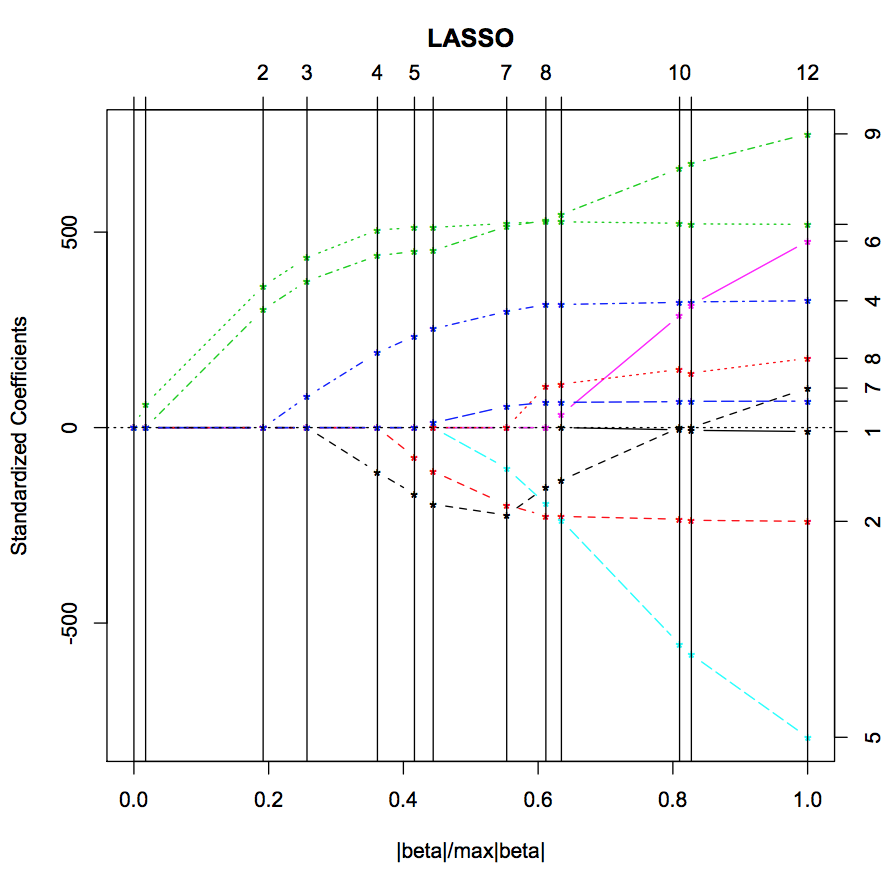
\includegraphics[width=0.75\textwidth]{img/lasso_path.png}
	\caption{Lasso coefficient solution path.}
\end{figure}

\subsubsection{Comments on the Lasso Estimator}

The Lasso estimator $\widehat {\bm \beta}$ is given by the solution to the unconstrained minimization problem
\begin{equation*}
	\widehat{\bm \beta} = \underset{{\bm \beta}}{\text{arg min~}} \left\{ \frac{1}{2} \| {\bf y} - {\bf X} {\bm \beta} \|^2_2 + \lambda \sum^p_{j = 1} |\beta_j| \right\}
\end{equation*}

Note that
\begin{itemize}
	\item The solution $\widehat {\bm \beta}$ varies continuously with the $\lambda$-convexity of the objective function.
	
	\item There are a sequence of $\lambda$'s which we call {\em transition points}, and the support of $\widehat {\bm \beta}$ stays locally constant between two adjacent transition points.
	
	\item The signs of the non-zero elements of $\widehat {\bm \beta}$ stays locally constant when $\lambda$ is between two transition points.
	
	\item For any given $\lambda$, the probability that $\lambda$ is a transition point is zero. That is, the set of transition points along $\R^+$ is of measure zero.
\end{itemize}

\subsection{Theoretical Considerations for the Lasso Estimator}

Define $A$ to be the {\em active set} of coefficients
\begin{equation*}
	A = \left\{ j\,:\, \widehat{\bm \beta} \neq 0 \right\},
\end{equation*}

and $S_A$ to be the {\em signs} of the elements of $A$
\begin{align*}
	S_A &= \left(s_j\right),~ j \in A, \quad \text{for} \\
	s_j &= \text{sign} \left( \widehat {\bm \beta}_j \right).
\end{align*}

Then, write $\widehat {\bm \beta} = \left(\widehat {\bm \beta}_A., 0\right)$. The solution $\widehat {\bm \beta}_A$ satisfies 
\begin{equation*}
	-{\bf X}^T_A \left({\bf y} - {\bf X}_A \widehat {\bm \beta}_A \right) + \lambda S_A = 0
\end{equation*}

which implies
\begin{align*}
	\widehat {\bm \beta}_A &= \left({\bf X}^T_A {\bf X}_A  \right)^{-1} \left({\bf X}_A  {\bf y} - \lambda S_A\right) \\
	&= \left({\bf X}^T_A {\bf X}_A  \right)^{-1} {\bf X}_A  {\bf y} - \lambda \left({\bf X}^T_A {\bf X}_A  \right)^{-1} S_A  \\
\implies \frac{d \widehat {\bm \beta}_A}{d\lambda} &= -\left({\bf X}^T_A {\bf X}_A  \right)^{-1} S_A.
\end{align*}

The above relation holds over the interval between two transition points since the solution path of $\widehat{\bm beta}$ is continuous between transition points. This result implies that the Lasso solution paths are piecewise linear (piecewise between transition points).

Next, the residuals ${\bf y} - \widehat{\bf y}$ are given by
\begin{equation*}
	{\bf y} - \widehat{\bf y} = {\bf y} - {\bf X}_A \left( {\bf X}^T_A {\bf X}_A \right)^{-1} {\bf X}^T_A {\bf y} + \lambda {\bf X}_A \left( {\bf X}^T_A {\bf X}_A \right)^{-1} S_A.
\end{equation*}	

Thus, taking the derivative of the residuals ${\bf y} - \widehat{\bf y}$ with respect to $\lambda$ yields
\begin{align*}
	\frac{d \left({\bf y} - \widehat{\bf y}\right)}{d\lambda} &= {\bf X}_A \left( {\bf X}^T_A {\bf X}_A \right)^{-1} S_A \\
	&= V_A.
\end{align*}

Note that $V_A$ is a special vector because
\begin{align*}
	{\bf X}^T_A V_A &= {\bf X}^T_A {\bf X}_A \left( {\bf X}^T_A {\bf X}_A \right)^{-1} S_A \\
	&= S_A.
\end{align*}

That is, ${\bf X}^T_A$ projects $V_A$ to the signs of the active set, $S_A$, i.e., for each $j \in A$, the inner product between $X_j$ and $V_A$ is either $+1$ or $-1$ (depending on the sign of the corresponding solution $\widehat \beta_j$). Note that $V_A$ was the derivative of the residual vector with respect to $\lambda$, and so the residual vector moves along a direction with equal angle with respect to all active covariates.

\section*{References}
\beginrefs
\bibentry{B95}{\sc L.~Breiman},``Better subset regression using the nonnegative garrote,''{\it Technometrics}, 37.4, 1995, pp.~373-384.
\bibentry{DJ95}{\sc D.L.~Donoho} and {\sc I.M.~Johnstone},``Adaptive to unknown smoothness via wavelet shrinkage,''{\it Journal of the american statistical association}, 90.432, 1995, pp.~1200-1224.
\bibentry{T96}{\sc R.~Tibshirani},``Regression shrinkage and selection via the lasso,''{\it Journal of the Royal Statistical Society. Series B (Methodological)}, 1996, pp.~267-288.
\bibentry{F98}{\sc W.J.~Fu},``Penalized regressions: the bridge versus the lasso,''{\it Journal of the computational and graphical statistics}, 7.3, 1998, pp.~397-416.
\bibentry{OPB00}{\sc M.R.~Osborne} and {\sc B.~Presnell} and {\sc B.A.~Turlach},``A new approach to variable selection in least squares,''{\it IMA journal of numerical analysis}, 20.3, 2000, pp.~389-403. 
\bibentry{EHJT04}{\sc B.~Efron} and {\sc T.~Hastie} and {\sc I.~Johnston} and {\sc R.~Tibshirani},``Least angle regression,''{\it The Annals of Statistics}, 32.2, pp.~407-499.
\bibentry{MR04}{\sc D.~Madigan} and {\sc G.Ridgeway},``[Least Angle Regression]: Discussion,''{\it The Annals of Statistics}, 32.2, 2004, pp.~465-469.
\bibentry{FHT10}{\sc J.~Friedman} and {\sc T.~Hastie} and {\sc R.~Tibshirani},``Regularization paths for generalized linear models via coordinate descent'',{\it Journal of statistical software}, 33.1, 2010, pp.~1.
\bibentry{YZ15}{\sc Y.~Yang} and {\sc H.~Zou},``A Fast Unified Algorithm for Solving Group-Lasso Penalized Learning Problems'',{\it Statistics and Computing}, 25.6, 2015, pp.~1129-141.
\endrefs


\end{document}





